% (c) 2026 Stephanie Märklin, OST Ostschweizer Fachhochschule
%
% !TEX root = ../../buch.tex
% !TEX encoding = UTF-8
%
% Rolle im Paper: Das Ergebnis der Rechnung formulieren und mathematisch deuten
%
% Stichworte:
% 17.5 Interpretation der Eigenwerte (Vorspann)
% - Andocken: die Rechnung liefert vier Zahlen -- jetzt ihre Deutung
% - Fahrplan: Real- und Imaginärteil, dann das komplexe Paar der
%   Dutch Roll
%
% 17.5.1 Realteil und Imaginärteil
% - Eigenwert zerlegen: lambda = sigma + i omega
% - e^{lambda t} in zwei Faktoren; Euler zitieren (Buchteil, DGL)
% - benennen: e^{sigma t} = Dämpfung (Vorzeichen offen),
%   Klammer = Schwingung mit Frequenz omega
% - Abbildung: drei Fälle sigma < 0, = 0, > 0 (TikZ aus Folien)
% - allgemeine Lösung als Linearkombination der vier Basislösungen;
%   Störung legt Anteile fest
% - keine Bewertung, kein Kriterium als Formel (Mechanik + Resultat)
%
% 17.5.2 Das komplexe Eigenwertpaar der Dutch Roll
% - reelle Matrix -> konjugierte Paare
% - Paar setzt sich zur reellen Schwingung zusammen (Buchteil)
% - reeller Eigenwert vs. komplexes Paar
% - Dutch Roll = komplexes Paar; klingt genau dann ab, wenn sigma < 0

\section{Interpretation der Eigenwerte
\label{aircraft:section:5-interpretation}}
\kopfrechts{Interpretation}
Die Rechnung des letzten Abschnitts liefert vier Zahlen.
In diesem Abschnitt deuten wir sie.
Wir betrachten zuerst Real- und Imaginärteil eines einzelnen
Eigenwerts, danach das komplexe Eigenwertpaar der Dutch Roll.

\subsection{Realteil und Imaginärteil
\label{aircraft:subsection:realteil-imaginaerteil}}
Wir schreiben einen Eigenwert als
\begin{equation}
    \lambda
    =
    \sigma + i\omega
    \label{aircraft:eqn:zerlegung}
\end{equation}
mit dem Realteil $\sigma$ und dem Imaginärteil $\omega$.
Die zugehörige Lösung zerfällt in zwei Faktoren,
\begin{equation}
    e^{\lambda t}
    =
    e^{\sigma t} \cdot e^{i\omega t}.
    \label{aircraft:eqn:faktoren}
\end{equation}
Mit der Eulerschen Formel aus Kapitel~\ref{...} ist
\begin{equation}
    e^{\lambda t}
    =
    e^{\sigma t} (\cos\omega t + i\sin\omega t).
    \label{aircraft:eqn:euler}
\end{equation}
Der Faktor $e^{\sigma t}$ ist die \emph{Dämpfung}, die Klammer die
\emph{Schwingung} mit der Frequenz $\omega$.
Die Abbildung~\ref{aircraft:fig:eigenwerte} zeigt die drei Fälle
$\sigma < 0$, $\sigma = 0$ und $\sigma > 0$.

\begin{figure}
    \centering
    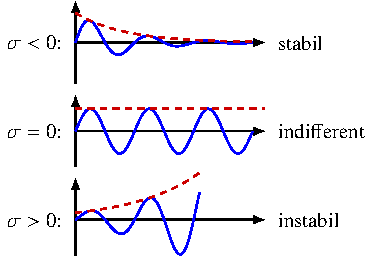
\includegraphics{papers/aircraft/images/eigenwerte.pdf}
    \caption{Die drei möglichen Verläufe von $e^{\lambda t}$ in
    Abhängigkeit vom Realteil $\sigma$ des Eigenwerts.
    Die gestrichelte Hüllkurve $e^{\sigma t}$ ist die Dämpfung, die
    Schwingung darin hat die Frequenz $\omega$.
    Nur für $\sigma < 0$ kehrt die Bewegung in die Ruhelage zurück.
    \label{aircraft:fig:eigenwerte}}
\end{figure}

Die allgemeine Lösung der Bewegungsgleichung ist eine
Linearkombination der vier Lösungen $\vec{x}_0^{(k)} e^{\lambda_k t}$,
und die Störung legt die Anteile fest.

\subsection{Das komplexe Eigenwertpaar der Dutch Roll
\label{aircraft:subsection:eigenwertpaar}}
Die Systemmatrix ist reell, also treten komplexe Eigenwerte als
konjugierte Paare $\sigma \pm i\omega$ auf.
Die beiden Lösungen eines Paars setzen sich nach
Kapitel~\ref{chapter:differentialgleichungen} zur reellen Schwingung
$e^{\sigma t}\cos\omega t$ zusammen.
Ein reeller Eigenwert beschreibt eine Bewegung ohne Schwingung, ein
komplexes Paar eine Schwingung mit der Dämpfung $\sigma$ und der
Frequenz $\omega$.
Die Dutch Roll ist ein komplexes Eigenwertpaar.
Sie klingt genau dann ab, wenn $\sigma < 0$ ist.